% GNUPLOT: LaTeX picture with Postscript
\documentclass{minimal}
% Set font size
\makeatletter
\def\@ptsize{1}
\InputIfFileExists{size11.clo}{}{%
   \GenericError{(gnuplot) \space\space\space\@spaces}{%
      Gnuplot Error: File `size11.clo' not found! Could not set font size%
   }{See the gnuplot documentation for explanation.%
   }{For using a font size a file `size<fontsize>.clo' has to exist.
        Falling back ^^Jto default fontsize 10pt.}%
  \def\@ptsize{0}
  \input{size10.clo}%
}%
\makeatother
\renewcommand*\rmdefault{cmss}%
% Load packages
\usepackage{calc}
\usepackage{graphicx}
\usepackage{color}
\usepackage{ucs}
\usepackage[utf8x]{inputenc}
\makeatletter
% Select an appropriate default driver (from TeXLive graphics.cfg)
\begingroup
  \chardef\x=0 %
  % check pdfTeX
  \@ifundefined{pdfoutput}{}{%
    \ifcase\pdfoutput
    \else
      \chardef\x=1 %
    \fi
  }%
  % check VTeX
  \@ifundefined{OpMode}{}{%
    \chardef\x=2 %
  }%
\expandafter\endgroup
\ifcase\x
  % default case
  \PassOptionsToPackage{dvips}{geometry}
\or
  % pdfTeX is running in pdf mode
  \PassOptionsToPackage{pdftex}{geometry}
\else
  % VTeX is running
  \PassOptionsToPackage{vtex}{geometry}
\fi
\makeatother
% Set papersize
\usepackage[papersize={360.00bp,216.00bp},text={360.00bp,216.00bp}]{geometry}
% No page numbers and no paragraph indentation
\pagestyle{empty}
\setlength{\parindent}{0bp}%
% Load configuration file
\InputIfFileExists{gnuplot.cfg}{%
  \typeout{Using configuration file gnuplot.cfg}%
}{%
 \typeout{No configuration file gnuplot.cfg found.}%
}%
%
\begin{document}
\begingroup
  \makeatletter
  \providecommand\color[2][]{%
    \GenericError{(gnuplot) \space\space\space\@spaces}{%
      Package color not loaded in conjunction with
      terminal option `colourtext'%
    }{See the gnuplot documentation for explanation.%
    }{Either use 'blacktext' in gnuplot or load the package
      color.sty in LaTeX.}%
    \renewcommand\color[2][]{}%
  }%
  \providecommand\includegraphics[2][]{%
    \GenericError{(gnuplot) \space\space\space\@spaces}{%
      Package graphicx or graphics not loaded%
    }{See the gnuplot documentation for explanation.%
    }{The gnuplot epslatex terminal needs graphicx.sty or graphics.sty.}%
    \renewcommand\includegraphics[2][]{}%
  }%
  \providecommand\rotatebox[2]{#2}%
  \@ifundefined{ifGPcolor}{%
    \newif\ifGPcolor
    \GPcolortrue
  }{}%
  \@ifundefined{ifGPblacktext}{%
    \newif\ifGPblacktext
    \GPblacktextfalse
  }{}%
  % define a \g@addto@macro without @ in the name:
  \let\gplgaddtomacro\g@addto@macro
  % define empty templates for all commands taking text:
  \gdef\gplbacktext{}%
  \gdef\gplfronttext{}%
  \makeatother
  \ifGPblacktext
    % no textcolor at all
    \def\colorrgb#1{}%
    \def\colorgray#1{}%
  \else
    % gray or color?
    \ifGPcolor
      \def\colorrgb#1{\color[rgb]{#1}}%
      \def\colorgray#1{\color[gray]{#1}}%
      \expandafter\def\csname LTw\endcsname{\color{white}}%
      \expandafter\def\csname LTb\endcsname{\color{black}}%
      \expandafter\def\csname LTa\endcsname{\color{black}}%
      \expandafter\def\csname LT0\endcsname{\color[rgb]{1,0,0}}%
      \expandafter\def\csname LT1\endcsname{\color[rgb]{0,1,0}}%
      \expandafter\def\csname LT2\endcsname{\color[rgb]{0,0,1}}%
      \expandafter\def\csname LT3\endcsname{\color[rgb]{1,0,1}}%
      \expandafter\def\csname LT4\endcsname{\color[rgb]{0,1,1}}%
      \expandafter\def\csname LT5\endcsname{\color[rgb]{1,1,0}}%
      \expandafter\def\csname LT6\endcsname{\color[rgb]{0,0,0}}%
      \expandafter\def\csname LT7\endcsname{\color[rgb]{1,0.3,0}}%
      \expandafter\def\csname LT8\endcsname{\color[rgb]{0.5,0.5,0.5}}%
    \else
      % gray
      \def\colorrgb#1{\color{black}}%
      \def\colorgray#1{\color[gray]{#1}}%
      \expandafter\def\csname LTw\endcsname{\color{white}}%
      \expandafter\def\csname LTb\endcsname{\color{black}}%
      \expandafter\def\csname LTa\endcsname{\color{black}}%
      \expandafter\def\csname LT0\endcsname{\color{black}}%
      \expandafter\def\csname LT1\endcsname{\color{black}}%
      \expandafter\def\csname LT2\endcsname{\color{black}}%
      \expandafter\def\csname LT3\endcsname{\color{black}}%
      \expandafter\def\csname LT4\endcsname{\color{black}}%
      \expandafter\def\csname LT5\endcsname{\color{black}}%
      \expandafter\def\csname LT6\endcsname{\color{black}}%
      \expandafter\def\csname LT7\endcsname{\color{black}}%
      \expandafter\def\csname LT8\endcsname{\color{black}}%
    \fi
  \fi
    \setlength{\unitlength}{0.0500bp}%
    \ifx\gptboxheight\undefined%
      \newlength{\gptboxheight}%
      \newlength{\gptboxwidth}%
      \newsavebox{\gptboxtext}%
    \fi%
    \setlength{\fboxrule}{0.5pt}%
    \setlength{\fboxsep}{1pt}%
    \definecolor{tbcol}{rgb}{1,1,1}%
\begin{picture}(7200.00,4320.00)%
    \gplgaddtomacro\gplbacktext{%
      \csname LTb\endcsname%%
      \put(864,3516){\makebox(0,0){\strut{}1}}%
      \put(1584,3516){\makebox(0,0){\strut{}0.1}}%
      \put(2303,3516){\makebox(0,0){\strut{}0.01}}%
    }%
    \gplgaddtomacro\gplfronttext{%
      \csname LTb\endcsname%%
      \put(1726,3852){\makebox(0,0)[r]{\strut{}$\theta_H$}}%
      \put(360,4103){\makebox(0,0)[l]{\strut{}a)}}%
    }%
    \gplgaddtomacro\gplbacktext{%
    }%
    \gplgaddtomacro\gplfronttext{%
      \csname LTb\endcsname%%
      \put(721,1596){\makebox(0,0){\strut{}}}%
      \put(1147,1596){\makebox(0,0){\strut{}}}%
      \put(1572,1596){\makebox(0,0){\strut{}}}%
      \put(1997,1596){\makebox(0,0){\strut{}}}%
      \put(2423,1596){\makebox(0,0){\strut{}}}%
      \put(568,1996){\makebox(0,0)[r]{\strut{} 8}}%
      \put(568,2300){\makebox(0,0)[r]{\strut{}10}}%
      \put(568,2604){\makebox(0,0)[r]{\strut{}12}}%
      \put(568,2908){\makebox(0,0)[r]{\strut{}14}}%
      \put(153,2376){\rotatebox{-270.00}{\makebox(0,0){\strut{}pH}}}%
      \colorrgb{1.00,1.00,1.00}%%
      \put(1981,2376){\rotatebox{-71.53}{\makebox(0,0){\strut{}0V vs RHE}}}%
      \colorrgb{1.00,1.00,1.00}%%
      \put(979,2689){\makebox(0,0){\strut{}Rh}}%
    }%
    \gplgaddtomacro\gplbacktext{%
    }%
    \gplgaddtomacro\gplfronttext{%
      \csname LTb\endcsname%%
      \put(1147,401){\makebox(0,0){\strut{}-1.5}}%
      \put(1572,401){\makebox(0,0){\strut{}-1.0}}%
      \put(1997,401){\makebox(0,0){\strut{}-0.5}}%
      \put(1572,71){\makebox(0,0){\strut{}U vs SHE (V)}}%
      \put(568,801){\makebox(0,0)[r]{\strut{} 8}}%
      \put(568,1105){\makebox(0,0)[r]{\strut{}10}}%
      \put(568,1409){\makebox(0,0)[r]{\strut{}12}}%
      \put(568,1713){\makebox(0,0)[r]{\strut{}14}}%
      \put(153,1181){\rotatebox{-270.00}{\makebox(0,0){\strut{}pH}}}%
      \colorrgb{1.00,1.00,1.00}%%
      \put(1981,1181){\rotatebox{-71.53}{\makebox(0,0){\strut{}0V vs RHE}}}%
      \colorrgb{1.00,1.00,1.00}%%
      \put(979,1494){\makebox(0,0){\strut{}Ir}}%
    }%
    \gplgaddtomacro\gplbacktext{%
    }%
    \gplgaddtomacro\gplfronttext{%
      \csname LTb\endcsname%%
      \put(2995,2791){\makebox(0,0){\strut{}}}%
      \put(3420,2791){\makebox(0,0){\strut{}}}%
      \put(3845,2791){\makebox(0,0){\strut{}}}%
      \put(2416,3191){\makebox(0,0)[r]{\strut{}}}%
      \put(2416,3495){\makebox(0,0)[r]{\strut{}}}%
      \put(2416,3799){\makebox(0,0)[r]{\strut{}}}%
      \put(2416,4103){\makebox(0,0)[r]{\strut{}}}%
      \colorrgb{1.00,1.00,1.00}%%
      \put(3829,3571){\rotatebox{-71.53}{\makebox(0,0){\strut{}0V vs RHE}}}%
      \colorrgb{1.00,1.00,1.00}%%
      \put(2827,3884){\makebox(0,0){\strut{}Ni}}%
    }%
    \gplgaddtomacro\gplbacktext{%
    }%
    \gplgaddtomacro\gplfronttext{%
      \csname LTb\endcsname%%
      \put(2995,1596){\makebox(0,0){\strut{}}}%
      \put(3420,1596){\makebox(0,0){\strut{}}}%
      \put(3845,1596){\makebox(0,0){\strut{}}}%
      \put(2416,1996){\makebox(0,0)[r]{\strut{}}}%
      \put(2416,2300){\makebox(0,0)[r]{\strut{}}}%
      \put(2416,2604){\makebox(0,0)[r]{\strut{}}}%
      \put(2416,2908){\makebox(0,0)[r]{\strut{}}}%
      \colorrgb{1.00,1.00,1.00}%%
      \put(3829,2376){\rotatebox{-71.53}{\makebox(0,0){\strut{}0V vs RHE}}}%
      \colorrgb{1.00,1.00,1.00}%%
      \put(2827,2689){\makebox(0,0){\strut{}Pd}}%
    }%
    \gplgaddtomacro\gplbacktext{%
    }%
    \gplgaddtomacro\gplfronttext{%
      \csname LTb\endcsname%%
      \put(2995,401){\makebox(0,0){\strut{}-1.5}}%
      \put(3420,401){\makebox(0,0){\strut{}-1.0}}%
      \put(3845,401){\makebox(0,0){\strut{}-0.5}}%
      \put(3420,71){\makebox(0,0){\strut{}U vs SHE (V)}}%
      \put(2416,801){\makebox(0,0)[r]{\strut{}}}%
      \put(2416,1105){\makebox(0,0)[r]{\strut{}}}%
      \put(2416,1409){\makebox(0,0)[r]{\strut{}}}%
      \put(2416,1713){\makebox(0,0)[r]{\strut{}}}%
      \colorrgb{1.00,1.00,1.00}%%
      \put(3829,1181){\rotatebox{-71.53}{\makebox(0,0){\strut{}0V vs RHE}}}%
      \colorrgb{1.00,1.00,1.00}%%
      \put(2827,1494){\makebox(0,0){\strut{}Pt}}%
    }%
    \gplgaddtomacro\gplbacktext{%
    }%
    \gplgaddtomacro\gplfronttext{%
      \csname LTb\endcsname%%
      \put(4843,2791){\makebox(0,0){\strut{}}}%
      \put(5268,2791){\makebox(0,0){\strut{}}}%
      \put(5693,2791){\makebox(0,0){\strut{}}}%
      \put(4264,3191){\makebox(0,0)[r]{\strut{}}}%
      \put(4264,3495){\makebox(0,0)[r]{\strut{}}}%
      \put(4264,3799){\makebox(0,0)[r]{\strut{}}}%
      \put(4264,4103){\makebox(0,0)[r]{\strut{}}}%
      \colorrgb{0.00,0.00,0.00}%%
      \put(5677,3571){\rotatebox{-71.53}{\makebox(0,0){\strut{}0V vs RHE}}}%
      \colorrgb{0.00,0.00,0.00}%%
      \put(4675,3884){\makebox(0,0){\strut{}Ag}}%
    }%
    \gplgaddtomacro\gplbacktext{%
    }%
    \gplgaddtomacro\gplfronttext{%
      \csname LTb\endcsname%%
      \put(4843,1596){\makebox(0,0){\strut{}}}%
      \put(5268,1596){\makebox(0,0){\strut{}}}%
      \put(5693,1596){\makebox(0,0){\strut{}}}%
      \put(4264,1996){\makebox(0,0)[r]{\strut{}}}%
      \put(4264,2300){\makebox(0,0)[r]{\strut{}}}%
      \put(4264,2604){\makebox(0,0)[r]{\strut{}}}%
      \put(4264,2908){\makebox(0,0)[r]{\strut{}}}%
      \colorrgb{0.00,0.00,0.00}%%
      \put(5677,2376){\rotatebox{-71.53}{\makebox(0,0){\strut{}0V vs RHE}}}%
      \colorrgb{0.00,0.00,0.00}%%
      \put(4675,2689){\makebox(0,0){\strut{}Au}}%
    }%
    \gplgaddtomacro\gplbacktext{%
    }%
    \gplgaddtomacro\gplfronttext{%
      \csname LTb\endcsname%%
      \put(4843,401){\makebox(0,0){\strut{}-1.5}}%
      \put(5268,401){\makebox(0,0){\strut{}-1.0}}%
      \put(5693,401){\makebox(0,0){\strut{}-0.5}}%
      \put(5268,71){\makebox(0,0){\strut{}U vs SHE (V)}}%
      \put(4264,801){\makebox(0,0)[r]{\strut{}}}%
      \put(4264,1105){\makebox(0,0)[r]{\strut{}}}%
      \put(4264,1409){\makebox(0,0)[r]{\strut{}}}%
      \put(4264,1713){\makebox(0,0)[r]{\strut{}}}%
      \put(6531,1799){\makebox(0,0)[l]{\strut{}$10^{-8}$}}%
      \put(6531,2951){\makebox(0,0)[l]{\strut{}$10^{-6}$}}%
      \put(6531,4103){\makebox(0,0)[l]{\strut{}$10^{-4}$}}%
      \put(7053,2548){\rotatebox{-270.00}{\makebox(0,0)[r]{\strut{}$\theta_H$}}}%
      \colorrgb{0.00,0.00,0.00}%%
      \put(5677,1181){\rotatebox{-71.53}{\makebox(0,0){\strut{}0V vs RHE}}}%
      \colorrgb{0.00,0.00,0.00}%%
      \put(4675,1494){\makebox(0,0){\strut{}Cu}}%
    }%
    \gplbacktext
    \put(0,0){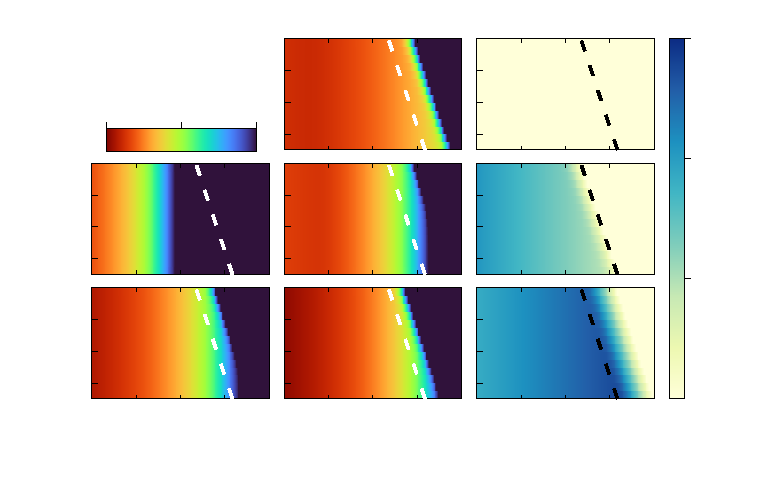
\includegraphics[width={360.00bp},height={216.00bp}]{Figure_Coverage_PeriodicTable-inc}}%
    \gplfronttext
  \end{picture}%
\endgroup
\end{document}
